% coding:utf-8

%----------------------------------------
%FOSADSVB, a LaTeX-Code for a summary of digital signal processing
%Copyright (C) 2015, Mario Felder & Michi Fallegger

%This program is free software; you can redistribute it and/or
%modify it under the terms of the GNU General Public License
%as published by the Free Software Foundation; either version 2
%of the License, or (at your option) any later version.

%This program is distributed in the hope that it will be useful,
%but WITHOUT ANY WARRANTY; without even the implied warranty of
%MERCHANTABILITY or FITNESS FOR A PARTICULAR PURPOSE.  See the
%GNU General Public License for more details.
%----------------------------------------

\chapter{Analog-Digital \& Digital-Analog Wandlung}
\section{Schritte der A/D- und D/A-Wandlung}
\paragraph{Sample:} Kontinuierliche Signalwerte werden mit der Samplefrequenz
$f_S$ aufgezeichnet. Dies erzeugt eine Sequenz von diskreten Signalwerten.

\paragraph{Quantize:} Die diskreten Signalwerte werden einer bestimmten
Anzahl Quantisierungsleveln zugeordnet.

\paragraph{Code:} Die quantisierten Abtastwerte können verwendet werden,
um die erhaltene Pulsfolge zu modulieren (Pulse Code Modulation PCM). Meistens
wird die Signalverarbeitung direkt mit den quantisierten Abtastwerten vorgenommen,
so dass diese ohne Modulation gespeichert werden. Dazu wird die Repräsentierung
der Quantisierungsleveln benötigt.\\
\\
Die Digital-Analog Wandlung enthält folgende Schritte:\\
\paragraph{Decode:} Die digitalen Werte werden in einer für die Digital-Analog
Wandlung repräsentativer Form benötigt.

\paragraph{Hold:} Das diskrete Signal muss über die Sampleperiode $T_S$ konstant
gehalten werden, ein Treppen ähnlicher Output entsteht.

\paragraph{Interpolate:} Das kontinuierliche Treppensignal wird durch Mittelwerte
von Tiefpass-Filtern geglättet.

\begin{center}
	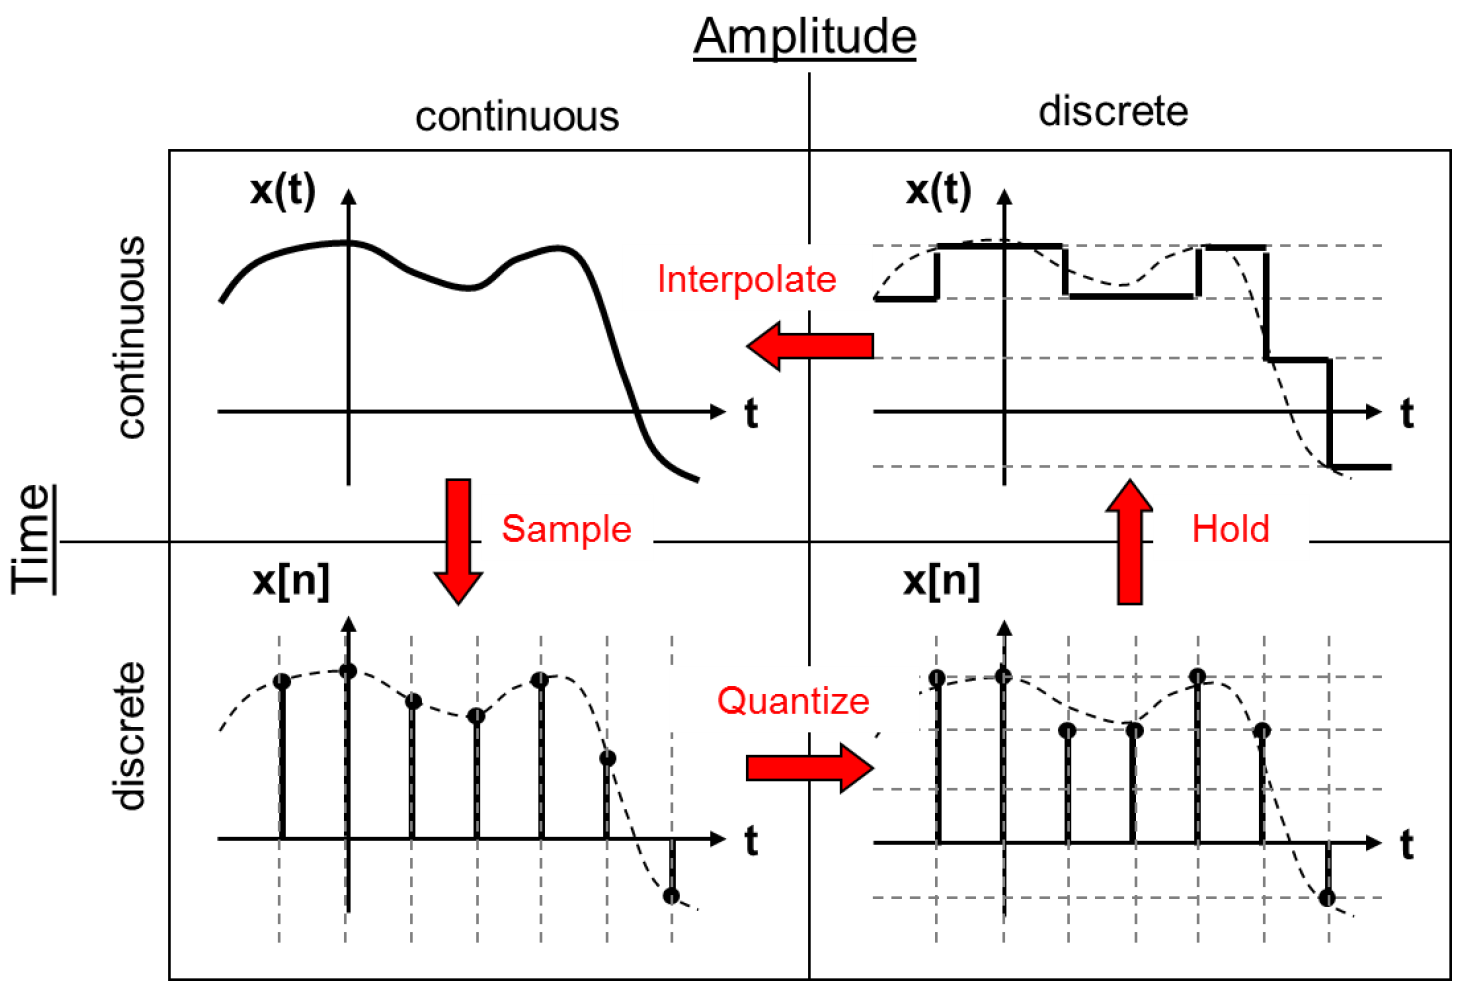
\includegraphics[scale=.7]{./images/ad_da}
\end{center}

%===============================================================================
\section{Abtasten und Aliasing}
\subsection{Abtasten von Tiefpass Signalen}
Mathematisch wird die Abtastung des Signals $x(t)$ durch eine Multiplikation
mit Dirac-Impulsen der Periode $T_S$ dargestellt:
\[ x_s(t) = \sum_{n=-\infty}^{\infty} x(t) \cdot \delta(t-nT_S) \]
Das Frequenzspektrum des abgetasteten Singals ist:
\[ X_S(f) = \frac{1}{T_S} \sum_{k)-\infty}^{\infty} X(f-kf_S) \]

\begin{center}
	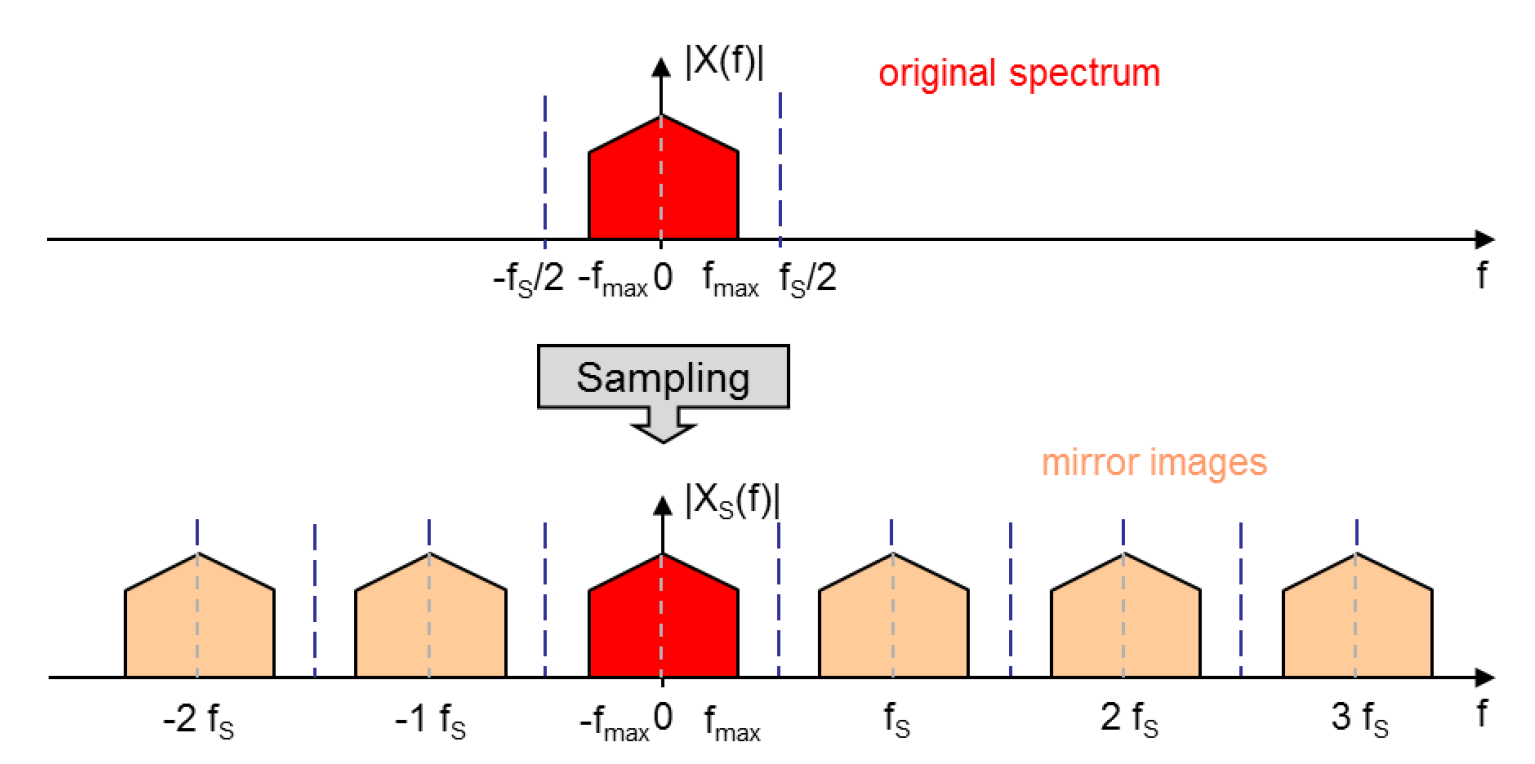
\includegraphics[scale=.7]{./images/frequenz_spectrum}
\end{center}
Um das Signal rekonstruieren zu können, müssen die Spiegelfrequenzen von $X(f)$
mit einem Tiefpassfilter unterdrückt werden. Das geht nur, wenn die grösste
Frequenz $f_{max}$ des Signals kleiner als die halbe Abtastfrequenz $f_S/2$ ist.
\[ f_S > 2 \cdot f_{max} \]

%===============================================================================
\subsection{Aliasing}
Aliasing entsteht, wenn das Abtasttheorem verletzt wird. Die Frequenzanteile
über $f_S/2$ werden in das Basisband gespiegelt und überlagern mit den 
gewünschten Frequenzen. Das analoge Signal kann nicht rekonstruiert werden.\\
\\
Dem kann mit einer Tiefpassfilterung entgegengewirkt werden. Der Filter hat
folgende Spezifikationen:
\[ f_{pass} \geq f_{desired} \]
\[ f_{stop} \leq f_S - f_{desire} \]

\begin{center}
	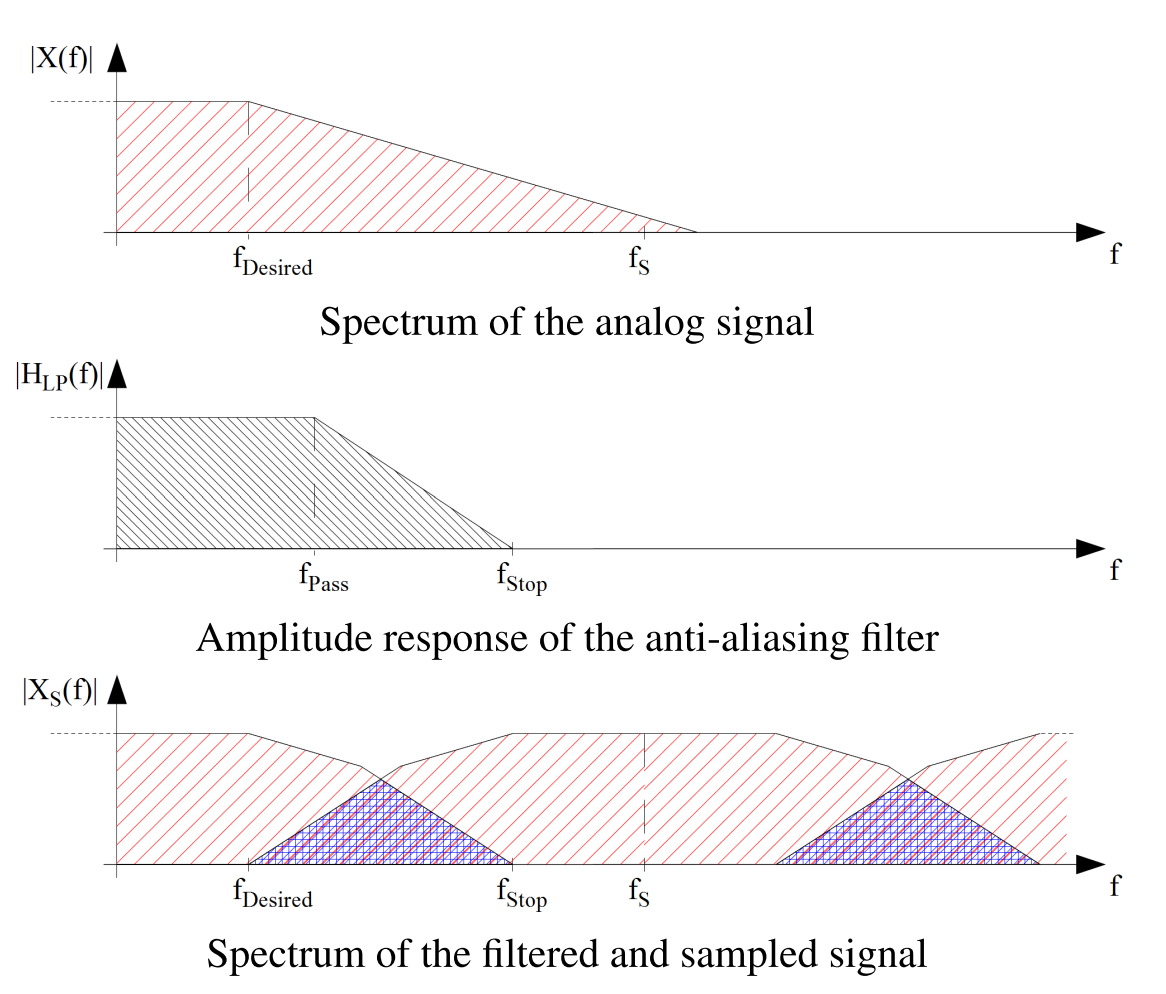
\includegraphics[scale=.7]{./images/aliasing}
\end{center}

%===============================================================================
\subsection{Abtasten von Bandpass Signalen}
Das Abtasttheorem wird folgendermassen angepasst (für $N\geq 1$):
\[ \frac{2\cdot f_{min}}{N} \geq f_S \geq \frac{2\cdot f_{max}}{N+1} \]
Für ungerade $N$ erscheint das originale Spektrum invertiert im Basisband.
Die originale Struktur des Spektrum wird zurückgewonnen durch invertierung
jedes zweiten Samples im Zeitbereich:
\[ \tilde{x}[n] = (-1)^n \cdot x[n] \]

\begin{minipage}{.5\textwidth}
	\begin{center}
		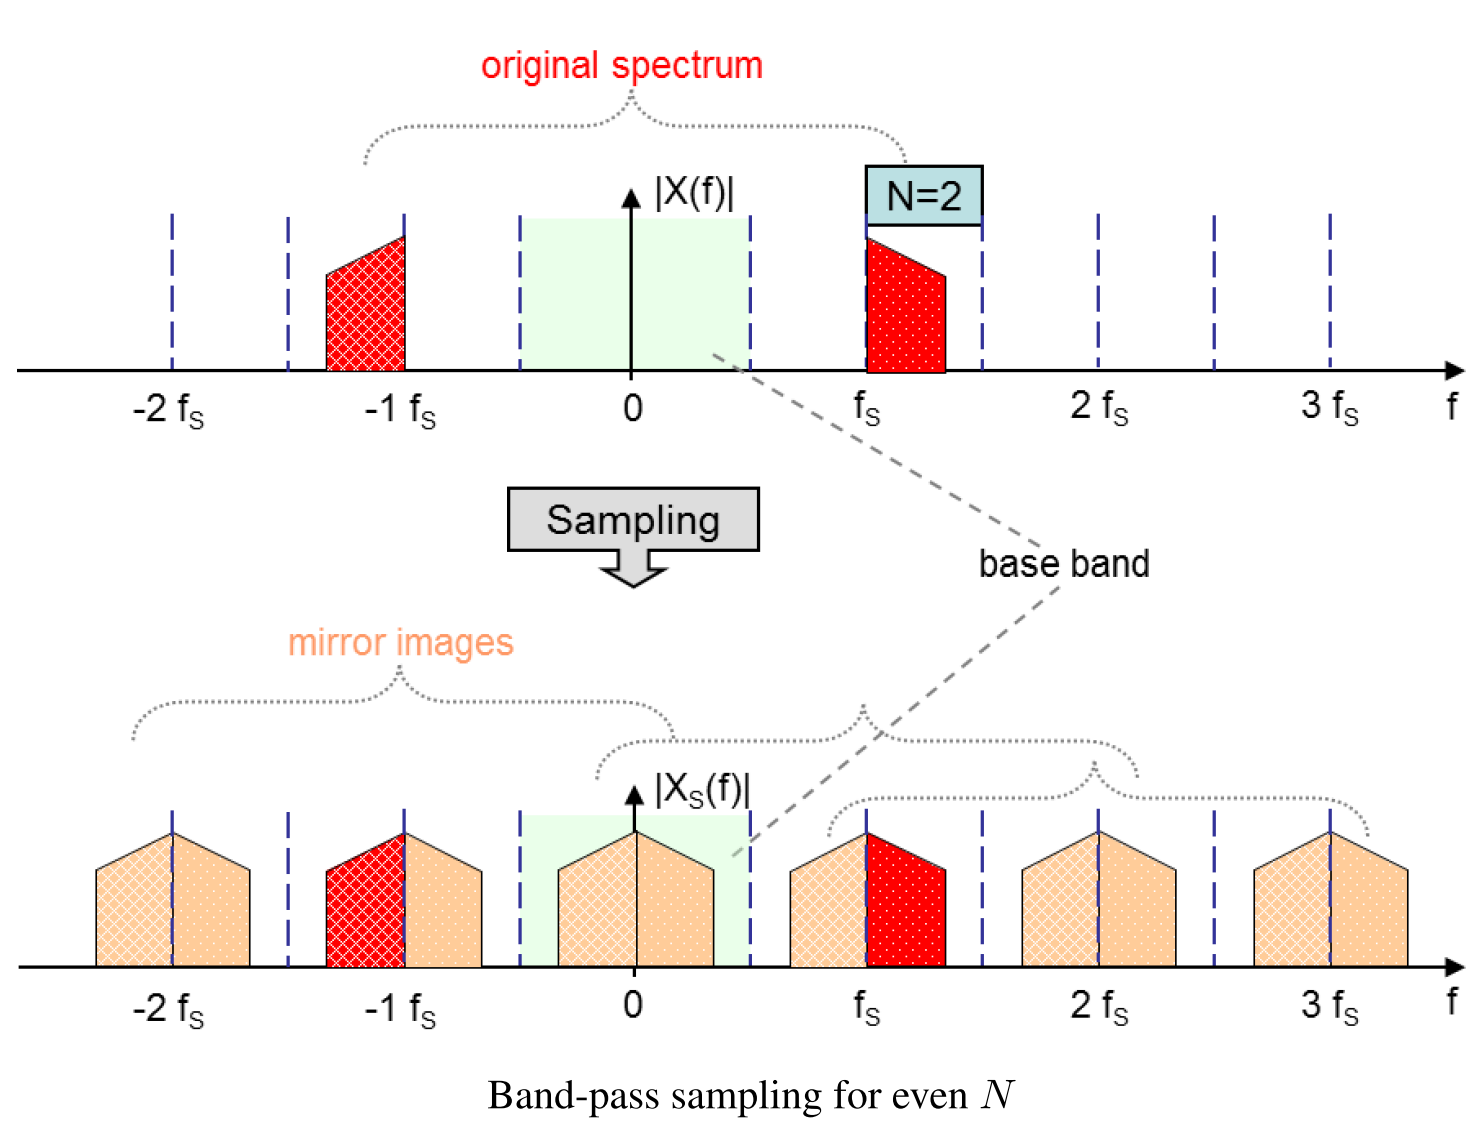
\includegraphics[width=\textwidth]{./images/bandpass_even}
	\end{center}
\end{minipage}
\begin{minipage}{.5\textwidth}
	\begin{center}
		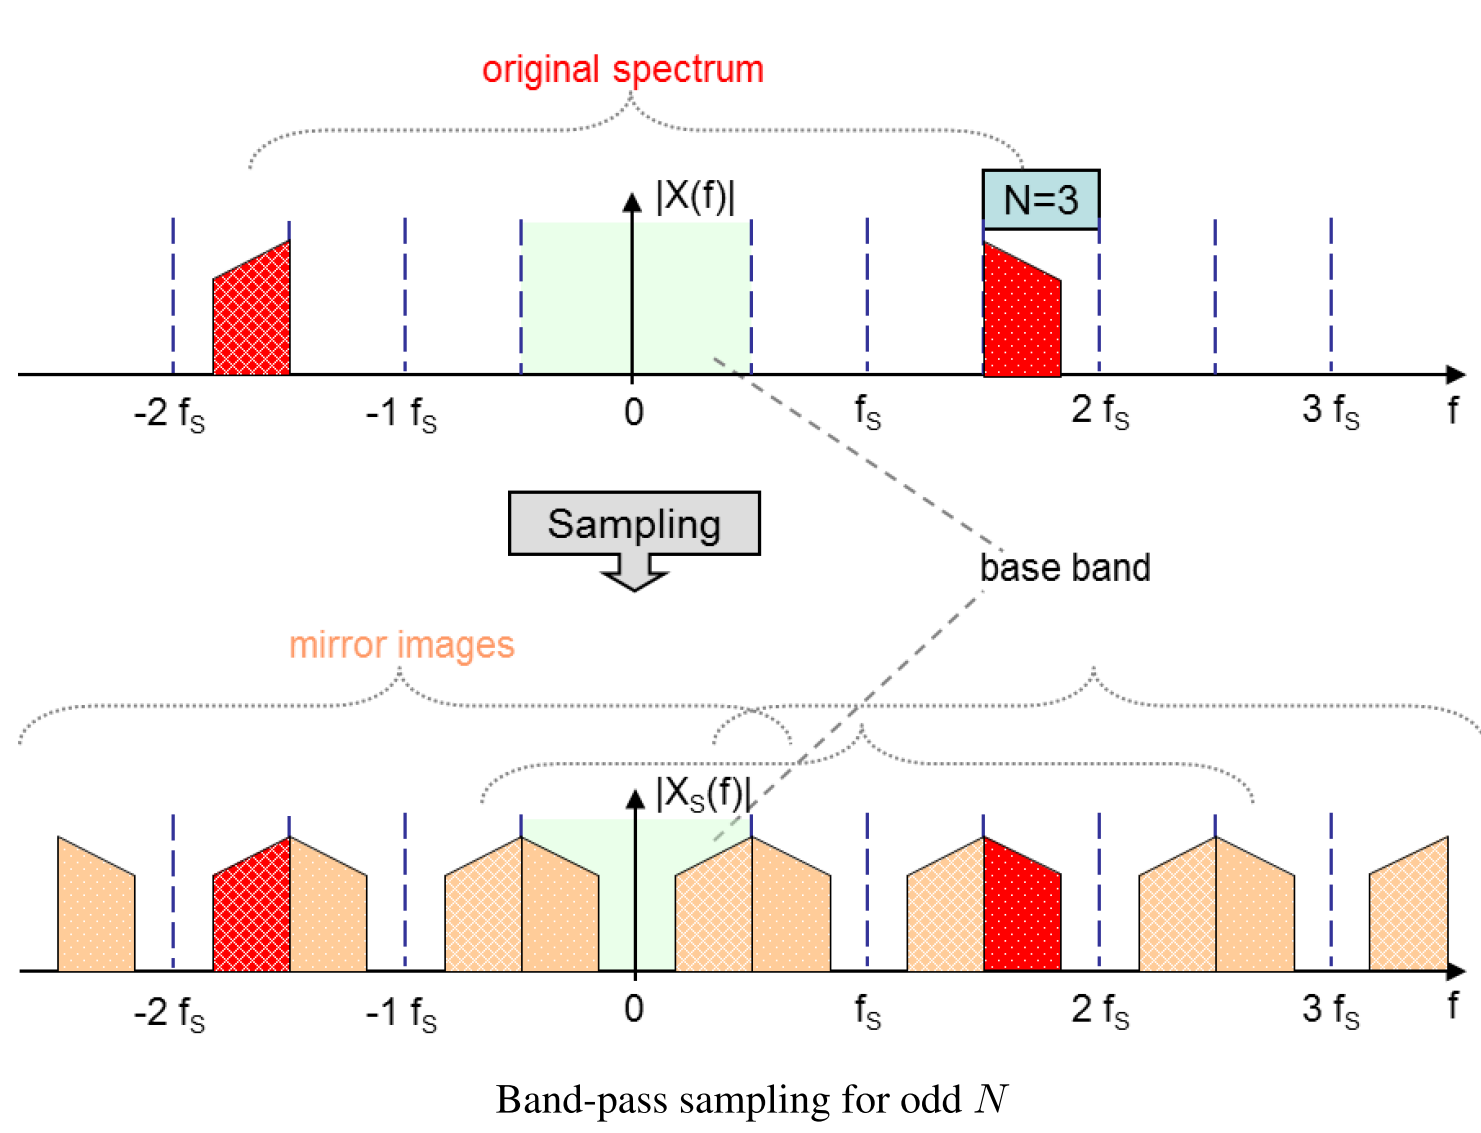
\includegraphics[width=\textwidth]{./images/bandpass_odd}
	\end{center}
\end{minipage}

%===============================================================================
\section{Quantisierung von Signalen}
\subsection{Uniforme Quantisierung}
Der Quantisierungsschritt (\textbf{quantization step}) $\Delta$ ist gegeben
durch die Auflösung mit $W$ bits und der dynamischen Reichweite $R$ des
abgetasteten Signals $x[n]$:
\[ \Delta = \frac{R}{2^W} \]
Durch das Abbilden eines amplitudenkontinuierlichen Signals auf eine endliche
Anzahl von Rekonstruktionsleveln können zweier Fehler entstehen:\\
\paragraph{Clipping:} Werte von $x[n]$ ausserhalb des Bereichs $R$ werden mit
dem maximum bzw. minimum Rekonstruktionslevel dargestellt.

\paragraph{Quantization error $\epsilon$:} Dieser Fehler tritt immer auf und
kann nicht verhindert werden. Die Grösse des Fehlers ist gegeben durch die
Qunatisierungsgrösse $\Delta$.\\

Für den mid-tread quantizer (runden zum nächsten Wert):
\[ -\Delta/2 < \epsilon \leq \Delta / 2 \]

Für den mid-rise quntizer:
\[ -\Delta < \epsilon \leq 0 \]

%===============================================================================
\subsection{Quantisierungsrauschen}
Der Quantisierungsfehler zeigt sich als Rauschen überlagert zum quantisierten
Signal:
\[ \epsilon[n] = x_q[n] - x[n] \]
Die Leistung $P_\epsilon$ des Quantisierungsrauschens
(\textbf{quantization noise}) ist:
\[ P_\epsilon = {\sigma_\epsilon}^2 = \int_{-\infty}^{\infty} (\epsilon - 
	{\sigma_\epsilon})^2 \cdot p(\epsilon) \di\epsilon = 
	\frac{\Delta^2}{12}\]
wobei $p(\epsilon)$ die Wahrscheinlichkeitsdichte ist. Angenommen die Werte
von $\epsilon[n]$ sind statistisch unkorreliert und uniform verteilt über den
Intervall $(-\Delta/2, \Delta/2]$ ist die Wahrscheinlichkeitsdichte für einen
mid-tread quantizer:
\[ p(\epsilon) = 1/\Delta \] 
Der Erwartungswert des Quantisierungsfehlers ist somit:
\[ \mu(\epsilon) = \int_{-\infty}^{\infty} \epsilon \cdot p(\epsilon) 
	\di\epsilon = \left. \frac{1}{2\Delta}\epsilon^2
	\right|_{-\Delta/2}^{\Delta/2} = 0 \]

\begin{center}
	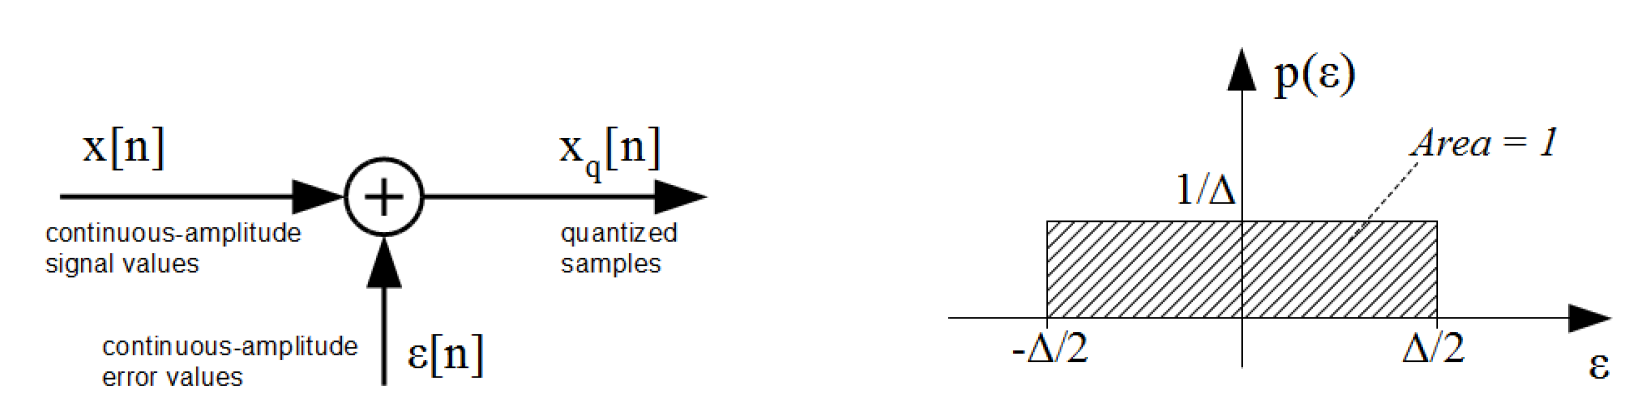
\includegraphics[width=.9\textwidth]{./images/quantization_noise}
\end{center}
Das SNR ist:
\[ SNR = \frac{P_x}{P_\epsilon} = 2^{2W} \cdot \frac{12P_x}{R^2} \]
\[\begin{aligned} SNR_{dB} &= 10 \cdot \left( \log_{10}2^{2W} +
	 \log_{10}\frac{12P_x}{R^2} \right)\\
	 &\approx 6W + 10 \cdot \log_{10}\frac{12P_x}{R^2} 
\end{aligned}\]
Bei einem harmonischen Inputsignal $x[n]$ ergibt sich folgendes SNR für
eine uniforme Quantisierung:
\[ SNR_{db} = 6W +1.76 \approx 6W \]